%%%%%%%%%%%%%%%%%%%%%%%%%%%%%%%%%%%%%%%%%
% Minimalist Book Title Page 
% LaTeX Template
% Version 1.0 (27/12/12)
%
% This template has been downloaded from:
% http://www.LaTeXTemplates.com
%
% Original author:
% Peter Wilson (herries.press@earthlink.net)
%
% License:
% CC BY-NC-SA 3.0 (http://creativecommons.org/licenses/by-nc-sa/3.0/)
% 
% Instructions for using this template:
% This title page compiles as is. If you wish to include this title page in 
% another document, you will need to copy everything before 
% \begin{document} into the preamble of your document. The title page is
% then included using \titleTH within your document.
%
%%%%%%%%%%%%%%%%%%%%%%%%%%%%%%%%%%%%%%%%%

%----------------------------------------------------------------------------------------
%	PACKAGES AND OTHER DOCUMENT CONFIGURATIONS
%----------------------------------------------------------------------------------------

%\title{Microprocessor Architecture : Labo 1}

\documentclass{article}

\usepackage[utf8]{inputenc}
\usepackage[T1]{fontenc}
\usepackage[svgnames]{xcolor} % Required to specify font color
\usepackage{mathpazo}
\usepackage{floatrow}
\usepackage{geometry}%réglages mise en page
\geometry{%
a4paper, % note : l'option a4paper tuait la marge supérieure.
body={170mm,250mm}, %
left=25mm,top=25mm,right=25mm, %
headheight=21mm,headsep=7mm,
marginparsep=4mm,
marginparwidth=20mm, %
footnotesep=50mm
}
\usepackage{longtable}
\usepackage{pdflscape}
% allows for temporary adjustment of side margins
\usepackage{chngpage}
\usepackage{graphicx}
\usepackage{float}
\usepackage{color}
\usepackage{amssymb}


\newcommand*{\course}{\fbox{PROJ-H-400}} % Generic publisher logo

%----------------------------------------------------------------------------------------
%	TITLE PAGE
%----------------------------------------------------------------------------------------

\newcommand*{\titleTH}{\begingroup % Create the command for including the title page in the document
\raggedleft % Right-align all text
\vspace*{\baselineskip} % Whitespace at the top of the page

{\Large \textsc{Anthony Debruyn}}\\[0.167\textheight] % Author name

{\LARGE\bfseries Year Project}\\[\baselineskip] % First part of the title, if it is unimportant consider making the font size smaller to accentuate the main title

{\textcolor{Purple}{\Huge Wysiwyd}}\\[\baselineskip] % Main title which draws the focus of the reader

{\Large \textit{The mobile wine cellar manager!}}\par % Tagline or further description

\vfill % Whitespace between the title block and the publisher

%\vspace*{30\baselineskip} % Whitespace at the bottom of the page

{\large Gaëtan Podevijn \course}\par % Publisher and logo

%\vspace*{5\baselineskip} % Whitespace at the bottom of the page
\endgroup}

%----------------------------------------------------------------------------------------
%	BLANK DOCUMENT
%----------------------------------------------------------------------------------------

\begin{document} 

\thispagestyle{empty}

\titleTH % This command includes the title page

\newpage

\section{Introduction}

\section{The Database}

\subsection{The Entity Relationship Diagram}

\begin{figure}[H]
\begin{center}
	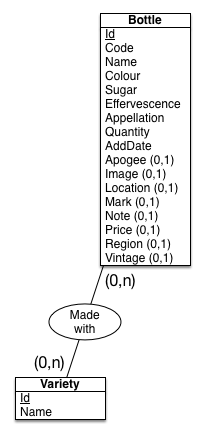
\includegraphics[scale=0.7]{../Entity Relationship DB diagram.png}
	\caption{The ERD.}
\end{center}
\end{figure}

\paragraph{Constraints}

\begin{itemize}
	\item If the type is "Champagne", then the Year attribute is not mandatory.
	\item The AddDate must be $\leq$ the current date.
	\item Id, Code, Quantity, Vintage, Apogee are a natural numbers.
	\item Price is a positive real number.
	\item Colour is a natural number in $\{ 0, 1, 2\}$.
	\item Sugar is a natural number in $\{0, 1, 2, 3\}$.
	\item Effervescence is a natural number in $\{0, 1, 2, 3\}$.
	\item Mark is a natural number in $\{0, 1, 2, 3, 4, 5\}$.
	\item Vintage is mandatory if the Effervescence attribute is set to "None".
\end{itemize}

\subsection{The Relational Model}

The translation of the ENR into the relational model:

\begin{description}
	\item[Bottle](\underline{Id}, Code, Name, Colour, Sugar, Effervescence, Appellation, Region, Vintage, Quantity, AddDate, \textit{Apogee}, \textit{Price}, \textit{Location}, \textit{Mark}, \textit{Image}, \textit{Note})
	
	\item[Variety](\underline{Id}, \underline{Name})
	
	\item[BottleVarieties](\underline{IdBottle, IdVariety})\\ \\
	\emph{BottleVarieties.IdBottle} foreign key to \emph{Bottle.Id}\\
	\emph{BottleVarieties.IdVariety} foreign key to \emph{Variety.Id}

\end{description}

\paragraph{Constraints}

\begin{itemize}
	\item If the type is "Champagne", then the Year attribute is not mandatory.
	\item The AddDate must be $\leq$ the current date.
	\item Id, Code, Quantity, Vintage, Apogee are a natural numbers.
	\item Price is a positive real number.
	\item Colour is a natural number in $\{ 0, 1, 2\}$.
	\item Sugar is a natural number in $\{0, 1, 2, 3\}$.
	\item Effervescence is a natural number in $\{0, 1, 2, 3\}$.
	\item Mark is a natural number in $\{0, 1, 2, 3, 4, 5\}$.
	\item Vintage is mandatory if the Effervescence attribute is set to "None".
\end{itemize}

\subsection{Normalisation}

\end{document}